\documentclass[main]{subfiles}
\begin{document}

%@@@@@@@@@@@@@@@@@@@@@@@@@@@@@@
% Main Topics: Membrane Potential 04.10.2018
% Lecturer: Valerio Mante
% author: Vanessa Leite - base document from benelot/eth-intro-to-neuroinformatics-summary

\section{Membrane Potential}

\subsection{Introduction}
In the lowest level, the brain process information in each processing unit (neurons) through membrane potential, molecules and ions.

Experiments in visual area of monkeys and cats (V1 recordings) allowed us to know more about the visual system. We now know that the visual system has orientation selectivity and the MT area respond to motion/velocity.

\href{https://www.youtube.com/watch?v=8VdFf3egwfg}{Here\footnote{https://www.youtube.com/watch?v=8VdFf3egwfg}} you can see an experiment and hear the neurons firing.

\begin{figure}[H]
	\centering
	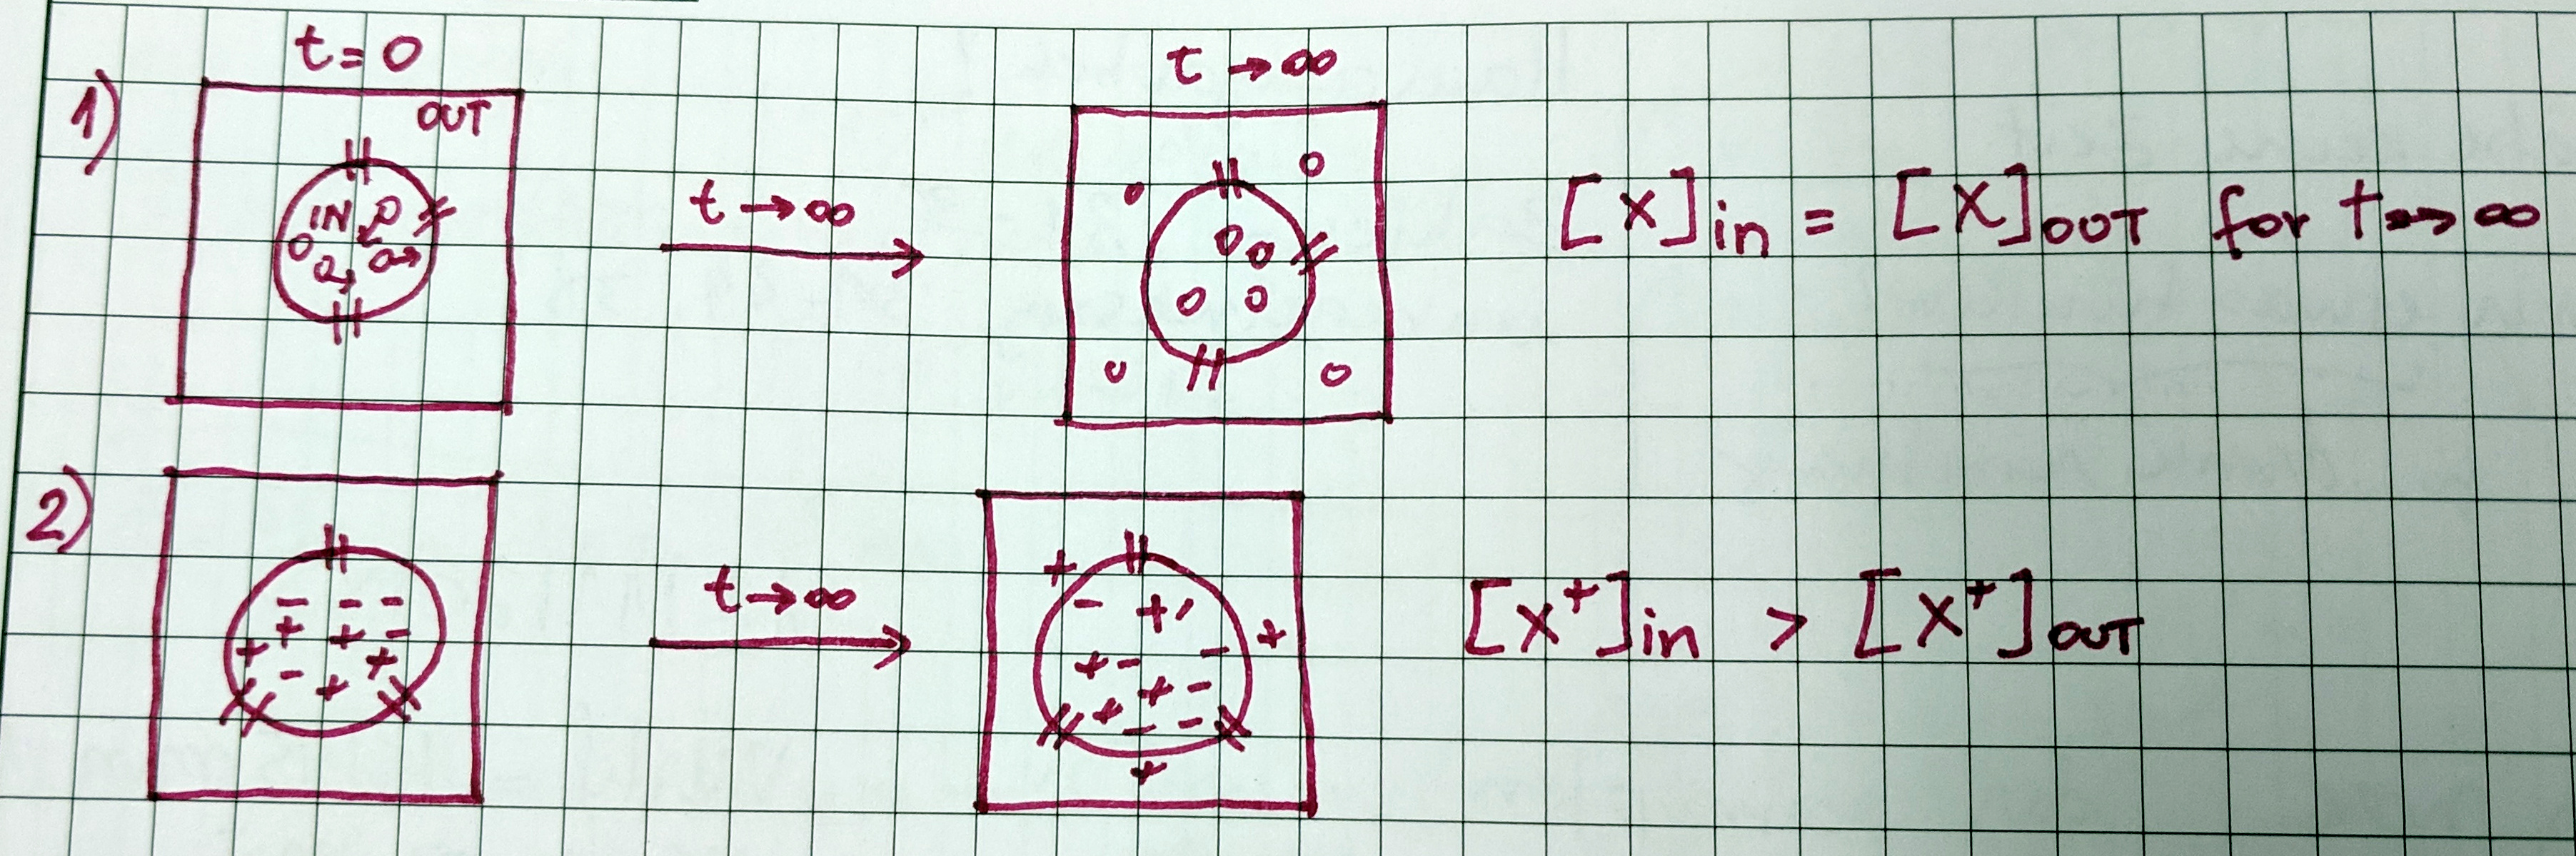
\includegraphics[width=0.7\textwidth]{membrane-potential-experiments.jpg}
	\caption{membrane potential experiments.}
	\label{fig:membrane-potential-experiments}
\end{figure}

Figure~\ref{fig:membrane-potential-experiments} shows two experiments of membrane potentia. In [1], $[X]_{in} = [X]_{out}$ for $t \to \infty$ because of diffusion. In a macroscopic point of view there is no change, microscopically, there is a constant change but on average we have a steady state.
In [2], however, we see pair os ions. Considering that the channels are selective for $+$, at $t=0$ we have no net charge ($\sum_+ + \sum_- = 0$). After a while, $+$ goes out and we have an excess charge on the surface and $[X^+]_{in} > [X^+]_{out}$ because the inside becomes negatively charged and thus "attractive" for the $+$ ($V_{in} < 0$). Thus, we have a net charge $V_{in} < V_{out}$.
Analogously, if the channels were selective for $-$, $[X^-]_{in} > [X^-]_{out}$, $V_{in} > V_{out}$.

This example has all the ingredients of the membrane potential in neurons:
\begin{itemize}
\item A physical barrier (in vs out)
\item $[X]_{in} \neq [X]_{out}$: different concentrations in/out
\item Selective channels
\end{itemize}

\subsection{Membrane structure}
\begin{itemize}[noitemsep,nolistsep]
	\item The membrane is a phospholipid bilayer and creates an energy barrier.
	\item Ions can not just flow through. Channels and pumps are needed.
	\item ECS: Extra cellular solution.
	\item ICS: Intra cellular solution.
	\item Membrane is built of two types of molecules, charged hydrophilic dipole head-group (outside) and an uncharged, hydrophobic hydrocarbon tail.
\end{itemize}

\subsection{Hyperpolarization}
\begin{itemize}[noitemsep,nolistsep]
	\item The extracellular space has potential $V=0\,mV$.
	\item The intracellular space has resting potential $V=-70\,mV$. Neurons at rest have their membrane potential mostly determined by $K^+$.
\end{itemize}

\subsection{Inputs to neurons, excitatory}
\begin{itemize}[noitemsep,nolistsep]
	\item Inputs to neurons over synapses.
	\item Depolarization, about $V=30\,mV$ presynaptic.
	\item Excitatory current is positive charge, which comes from the extra- to intra-cellular space.
	\item The signal is analog and graded.
	\item On the way to the soma, the intra-cellular current gets reduced by leak current (positive charge) that leaves the intra-cellular space.
	\item From the large depolarization ($V=0\,mV$), about $V=-69.5\,mV$ is the value at the soma.
	\item EPSP (excitatory postsynaptic potential) $0.2$ to $0.4\,mV$.
	\item Spatial and temporal spread of the signal.
	\item $\tau_m$ defines how fast potentials changes.
	\item $\lambda$ defines how far currents travel.
\end{itemize}

\begin{figure}[H]
	\centering
	\scalebox{0.7}{\includegraphics{spatial_temporal_spread.png}}
\end{figure}

\subsection{Chemical synapses}
\begin{figure}[H]
	\centering
	\scalebox{0.7}{\includegraphics{chemical_synapse.png}}
\end{figure}
\begin{itemize}[noitemsep,nolistsep]
	\item Digital transmission, but can have failures, and graded release.
	\item There can even be synapses directly on the soma or axon.
\end{itemize}

\subsection{Inhibitory post-synaptic potential}
\begin{itemize}[noitemsep,nolistsep]
	\item Depolarization, about $V=30\,mV$ presynaptic.
	\item A large hyperpolarization, $V=-90\,mV$ at postsynaptic dendrite.
	\item Small hyperpolarization at soma, $V=-70.2\,mV$.
\end{itemize}

\subsection{Summation of Inputs}
\begin{itemize}[noitemsep,nolistsep]
	\item Temporal summation, one input after another.
	\item Spatial summation, inputs from different dendrite branches.
	\item Summing up, the threshold is crossed.
	\item Typically 20 to 30 Inputs are needed to go above threshold.
	\item The action potential gets triggered at the beginning of the axon.
	\item The threshold is about $-60\,mV$.
\end{itemize}

\subsection{Action potential}
\begin{itemize}[noitemsep,nolistsep]
	\item Has an active regenerative process.
	\item The duration is about 1 to 2 ms.
	\item All-or-none (digital).
	\item Amplitude gets converted into rate.
	\item Components: Depolarization, overshoot ($>0\,mV$), repolarization/hyperpolarization and a refractory period (back to $-70\,mV$).
	\item Peak about $0.5\,ms$ long, $4.4\,ms$ refractory period.
\end{itemize}
\begin{figure}[H]
	\centering
	\begin{subfigure}[b]{0.5\textwidth}
		\centering
		\includegraphics[width=\textwidth]{voltage-source-in-membrane.png}
	\end{subfigure}%
	~
	\begin{subfigure}[b]{0.5\textwidth}
		\centering
		\includegraphics[width=\textwidth]{action_potential_01.png}
	\end{subfigure}
\end{figure}
\begin{figure}[H]
	\centering
	\begin{subfigure}[b]{0.5\textwidth}
		\centering
		\includegraphics[width=\textwidth]{voltage-source-in-membrane2.png}
	\end{subfigure}%
	~
	\begin{subfigure}[b]{0.5\textwidth}
		\centering
		\includegraphics[width=\textwidth]{action_potential_02.png}
	\end{subfigure}
\end{figure}

\subsection{Axon}
\begin{itemize}[noitemsep,nolistsep]
	\item Myelin sheet is often wrapped around the axon.
	\item This makes the white-matter white.
	\item Myelin is an electrical insulator which grants faster propagation.
	\item Less energy is needed with myelinated axons.
	\item The current goes through the node of ranvier (myelin sheath gaps).
\end{itemize}

\subsection{Ionic currents and equilibrium}
\subsubsection{Receptors:}
\begin{itemize}[noitemsep,nolistsep]
	\item Excitatory: AMPA/NDMA, mixed cation, $V(drive) =0\,mV$
	\item Inhibitory: GABA A, chloride (Cl), $V(drive) =-65\,mV$
	\item Inhibitory: GABA B, potassium (K), $V(drive) =-90\,mV$
\end{itemize}
\subsubsection{Action potential:}
\begin{itemize}[noitemsep,nolistsep]
	\item Sodium (Na): $V(drive) = 55\,mV$
	\item Potassium (K); $V(drive) = -90\,mV$
\end{itemize}

\subsubsection{Ion equilibrium}
\textbf{Charge carrier (giant squid axon)}:\\
\begin{tabular}{|l|l|l|l|}
	\hline
	Ion type & Cytoplasm (mM) & Extracellular (mM) & Equilibrium potential (mV)\\\hline
	$K^+$ & 400 & 20 & -75 \\\hline
	$Na^+$ & 50 & 440 & +55\\\hline
	$Cl^-$ & 52 & 560 & -60\\\hline
	$Ca^{2+}$ & 0.0001 & 10 & +140\\\hline
\end{tabular}
\begin{figure}[H]
	\centering
	\scalebox{0.5}{\includegraphics{bilayer-closeup2.png}}
\end{figure}

\subsection{Permeability equations}

\subsubsection{Acting forces}
\begin{itemize}[noitemsep,nolistsep]
	\item Ion concentration gradient (diffusion).
	\item Electric potential (electrostatic force).
	\item Both forces are in equilibrium in resting/passive state.
	\item Equilibrium potential can be computed with the Nernst equation.
	\item Neurons have $K^+$, $Na^+$ and $Cl^-$ channels.
	\item $K^+$ permeability is greater than $Na^+$ permeability.
	\item Active $Na^+$-$K^+$ pump creates an ion gradient. The exchange is 2 $K^+$ against 3 $Na^+$ ions.
	\item When a positively charged ion tries to go in, it is repelled by the potential in the membrane. So, the probability of the ion to get in depends of a constante times the amount of positive ions out.
\end{itemize}

\subsubsection{Nernst equation}
\[V_{eq} = \frac{K_BT}{qZ} \cdot \ln (\frac{[Ion]_{extracellular}}{[Ion]_{intracellular}})\]

\begin{itemize}[noitemsep,nolistsep]
	\item $K_B$: Boltzman constant.
	\item T: Absolute temperature (kelvin).
	\item qZ: charge of the ion
	\item $V_{eq}$: Voltage on equilibrium
	\item One mole has $6.022\cdot10^{23}$ ions, solution is one molar when its concentration is $1\,\frac{mol}{l}$.
	\item This equation doesnt take into account conductance or number of channels. This is because we are looking to the equilibrium state, so it doesn't matter.
	\item if temperature increases, the potential increases: more thermal energy thus more ions can cross the potential barrier
	\item if $|Z|$ increases, then potential decreases: (?) larger energy barrier ($\Delta E = qZV$).
	\item change in charge sign ($Z$) leads to change in potential sign
	\item dependent of concentration: $[X]_{out} > [X]_{in} \to V > 0$ $(Z > 0)$ and $[X]_{out} < [X]_{in} \to V < 0$ $(Z > 0)$
\end{itemize}

\subsubsection{Simplified equation}
\begin{itemize}[noitemsep,nolistsep]
	\item Take the temperature as $300K$.
	\item $K_B = 1.38 \times 10^{-23} \frac{J}{K}$
	\item $q = 1.60 \times 10^{-19} C$
	\item Replace $\ln$ with $\log$, gives a factor $2.3$.
\end{itemize}

\[\frac{K_BT}{q} \approx 24 - 27 mV\] for cold and warmed blood animals.

\begin{figure}[H]
	\centering
	\begin{subfigure}[b]{0.5\textwidth}
		\centering
		\includegraphics[width=\textwidth]{equilibrium_nernst_01.png}
	\end{subfigure}%
	~
	\begin{subfigure}[b]{0.3\textwidth}
		\centering
		\includegraphics[width=\textwidth]{membrane_potential.png}
	\end{subfigure}
\end{figure}

\subsubsection{Membrane capacitance}
Consider the capacitance of the membrane $Cm = \frac{c_m}{A}$, where $c_m$ is the specific capacitance and $A$ is the area. Consider $c_m \approx 10 \frac{nF}{mm^2}$, $A \approx 0.01 - 0.1 mm^2$, thus $Cm \approx 0.1 - 1 nF$.

\paragraph{How many ions are necessary to get $Vm = -70 mV$?}
$Cm = \frac{Qm}{Vm} \rightarrow Qm = Cm \times Vm = 10^{-9} \times 70 \times 10^{-3} C = 7 \times 10^{-11} C$.
Number of ions: $\frac{Qm}{q} = \frac{7\times 10^{-11}}{1.6 \times 10^{-19}} \rightarrow \approx 10^9$ ions.

\paragraph{How many ions there are in a neuron?}
Volume of a neuron is approximately $10^6 \mu m^3$, thus, contains $10^{14}$ ions

Only $1:10^5$ ions contribute to the membrane potential at rest. For each ion that moves, we need a lot that do not.
But, what if $Cm$ and $Qm \propto r^2$, $volume \propto r^3$: ratio $\propto \frac{1}{r}$.
What if potential $V \neq Veq$?

\begin{figure}[H]
	\centering
	\begin{subfigure}[b]{0.5\textwidth}
		\centering
		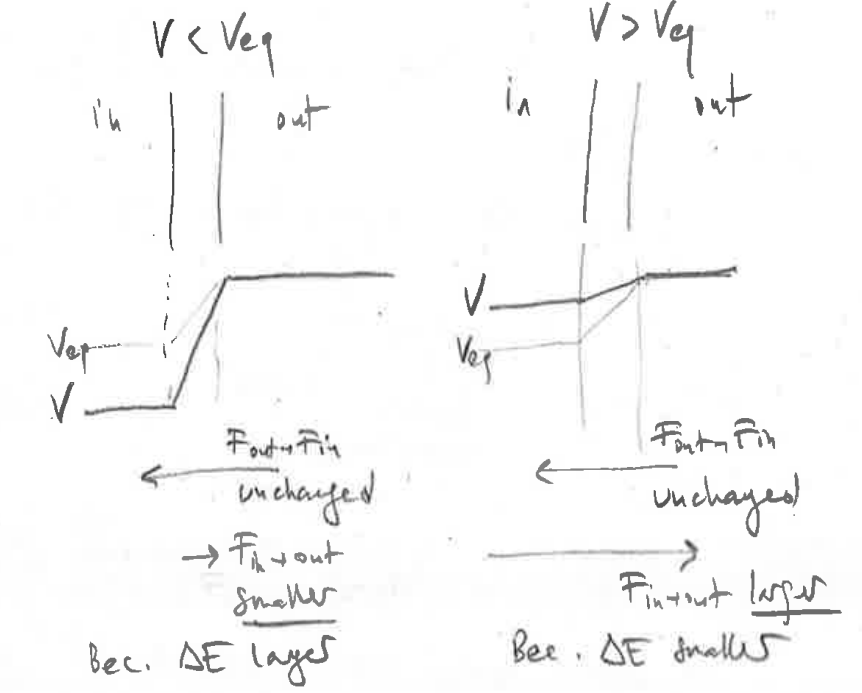
\includegraphics[width=\textwidth]{membrane-flow.png}
	\end{subfigure}%
	~
	\begin{subfigure}[b]{0.3\textwidth}
		\centering
		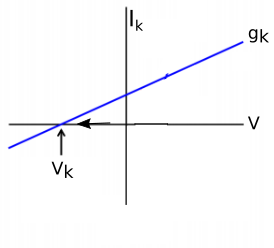
\includegraphics[width=\textwidth]{current_voltage_03.png}
	\end{subfigure}
	\caption{membrane flow}
	\label{fig:membrane-flow}
\end{figure}

Figure~\ref{fig:membrane-flow} shows the behavior for the case of a different potential. $I_k$ tries to pull $V$ towards $V_k$. The slope difference of $g_k$ tell us how much is necessary to pull until achieve the equilibrium.

\subsubsection{Goldmann-Equation}
\begin{itemize}[noitemsep,nolistsep]
	\item Nernst does not consider multiple ions and permeability.
	\item Goldmann describes membrane potential, with multiple ions and permeability.
	\item Assumes ion flux obeys Nernst/Planck equation.
	\item Assumes ions move across membrane independently, without interaction.
	\item Equilibrium: $P_K:P_{Na}:P_{Cl}$ is $1:0.04:0.45$.
	\item Action potential: $P_K:P_{Na}:P_{Cl}$ is $1:20:0.45$.
	\item $V_m$: Membrane potential.
	\item $P$: Membrane permeability.
	\item $[A^x]$: Ion concentration.
	\item New $V_eq$ depends on the conductance of the channels.
	\item $I_k$ is also called $I_L$ (leak). 
	\item Reverse potential that are bigger than $I_L$ leads to excitation and smaller leads to inhibition.
\end{itemize}

\[V_m = \frac{K_BT}{q} ln(\frac{P_K[K^+]_{out} + P_{Na}[Na^+]_{out} + P_{Cl}[Cl^{-}]_{in}}{P_K[K^+]_{in} + P_{Na}[Na^+]_{in} + P_{Cl}[Cl^{-}]_{out}})\]

\end{document}
